\section{Experimental Setup}\label{sec:appendix_Experimental}

This section provides a detailed overview of the experimental setup used in our study, including the pruning techniques, datasets, sparsity ranges, and computational environment.


We employed a range of established one-shot pruning techniques, which perform pruning in a single step, followed by Hessian-based updates of the remaining weights and reduce the impact on loss after pruning.
Specifically, we considered WoodFisher~\cite{WoodFisher}, CBS~\cite{CBS}, CHITA~\cite{CHITA}, and Matrix-Free Approximate Curvature (M-FAC)~\cite{mfac}. Performance metrics for these methods were sourced from existing literature~\cite{CBS,CHITA}, with results averaged over three independent runs.

\textbf{Application of \REFLOW{}:}  
In this work, \REFLOW{} is applied to networks pruned using \emph{magnitude pruning}. After pruning, Batch Normalization (BN) running statistics are recalibrated using a forward pass over a limited number of training samples. 

\textbf{Hyperparameters:}  
For \REFLOW{}, we used 50 training batches to recalibrate the running BN statistics, with a batch size of 128 across all experiments.

\textbf{Pre-Trained Networks and Datasets:}  
To ensure comparability with prior studies~\cite{CBS,CHITA}, we adopted datasets and model architectures from the same studies. The analysis included three pre-trained networks: ResNet-20~\cite{RESNET} trained on the CIFAR-10 dataset~\cite{CIFAR10}, and MobileNet~\cite{MobileNet} and ResNet-50~\cite{RESNET} trained on the ImageNet dataset~\cite{ImageNet}. 

We extended the analysis to include larger architectures that prior leading one-shot pruning methods~\cite{WoodFisher, CBS} did not explore and are unable to scale to efficiently. Specifically, we evaluated \REFLOW{} on ResNet-101~\cite{RESNET}, ResNet-152~\cite{RESNET}, RegNetX~\cite{radosavovic2020designing}, and ResNeXt-101~\cite{xie2017aggregated}, all trained on the ImageNet dataset.


\textbf{Sparsity Range:}  
We evaluated \REFLOW{} across the following sparsity ranges, consistent with prior works~\cite{CBS,CHITA}:
\begin{itemize}
    \item \textbf{ResNet-20 on CIFAR-10:} Sparsity range of 0.4 to 0.9.
    \item \textbf{MobileNet on ImageNet:} Sparsity range of 0.4 to 0.8.
    \item \textbf{ResNet-50 on ImageNet:} Sparsity range of 0.4 to 0.9.
\end{itemize}


\textbf{Hardware:}  
All experiments were conducted on a computational setup comprising an NVIDIA RTX A6000 GPU with 48GB memory, 10,752 CUDA cores, and 336 Tensor cores capable of 309 TFLOPS peak performance, coupled with an AMD EPYC 7713P 64-Core CPU.

\textbf{Software:}  
The computational environment operated on Ubuntu 20.04.6 LTS (Focal Fossa), utilizing Python version 3.8.10 and PyTorch version 2.1.0.






\section{Ablation Studies}\label{sec:appendix}
In this section, we evaluate the performance of \REFLOW{} through ablation studies. We analyze the impact of the number of training batches (\(N\)), layer-wise BN recalibration, and batch size on accuracy recovery in pruned networks.


\subsection{Effect of the Number of Training Batches on Performance}\label{sec:Ablation_batches}

We analyze the impact of varying the number of training batches (\(N\)) on the performance of \REFLOW{}, focusing on test accuracy. \REFLOW{} is applied to sparse networks after magnitude pruning, recalibrating Batch Normalization (BN) statistics through a forward pass over \(N\) training batches. 

Figure~\ref{fig:mobnet_accuracy_batches} shows the relationship between \(N\) and test accuracy for MobileNet at 80\% sparsity. Accuracy improves significantly for small values of \(N\), saturating around \(N = 50\). Using \(N = 50\) training batches with a batch size of 128 corresponds to only 6,400 images—less than 0.5\% of the 1.28 million training samples in ImageNet.

In contrast, leading impact-based pruning methods such as WoodFisher \cite{WoodFisher} and CBS \cite{CBS} require 960,000 training samples for gradient computation, while CHITA \cite{CHITA} requires 16,000 samples. \REFLOW{} achieves comparable performance using just 6,400 samples without any gradient computation, relying solely on forward passes to update BN statistics. This minimal data requirement enables \REFLOW{} to operate in scenarios where access to the full training dataset is limited, such as privacy-preserving applications or resource-constrained environments, where re-training is infeasible.



\begin{figure}[t]
\centering
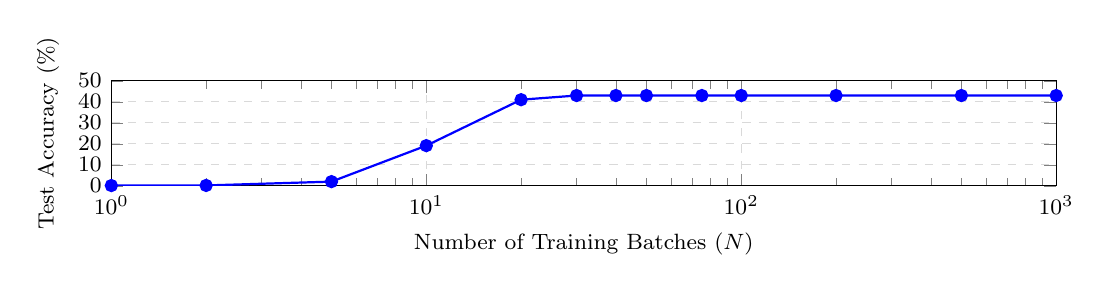
\begin{tikzpicture}
    \begin{semilogxaxis}[
        width=12cm,
        height=0.11\textwidth,
        scale only axis,
        grid=major,
        grid style={dashed,gray!30},
        tick label style={font=\footnotesize},
        label style={font=\footnotesize},
        legend style={font=\footnotesize},
        cycle list name=color list,
        legend cell align=left,
        xlabel={Number of Training Batches $(N)$},
        ylabel={Test Accuracy (\%)},
        xmin=1, xmax=1000,
        ymin=0, ymax=50,
        ytick={0, 10, 20, 30, 40, 50},
        log basis x={10}
    ]

    % MobileNet accuracy at 80% sparsity
    \addplot[color=blue, mark=*, solid, thick] coordinates {
        (1, 0.136)
        (2, 0.194)
        (5, 2.012)
        (10, 19.148)
        (20, 41.022)
        (30, 43)
        (40, 43)
        (50, 43)
        (75, 43)
        (100, 43)
        (200, 43)
        (500, 43)
        (1000, 43)
    };

    \end{semilogxaxis}
\end{tikzpicture}
\caption{Test accuracy of MobileNet at 80\% sparsity using \REFLOW{} for different numbers of training batches (\(N\)). Accuracy improves significantly for \(N \leq 20\), saturates around \(N = 50\), and stabilizes for larger \(N\).}\label{fig:mobnet_accuracy_batches}
\end{figure}


\subsection{Impact of Layer-wise Recovery on Performance}\label{sec:Ablation_layerwise}

To gain deeper insights into the recovery of test accuracy in sparse networks, we analyzed the contribution of individual Batch Normalization (BN) layers by recalibrating them sequentially. Specifically, the recalibration was performed one layer at a time, measuring the cumulative improvement in test accuracy after recalibrating each BN layer. This process was conducted in two directions: from the first BN layer to the last (forward direction) and from the last BN layer to the first (backward direction).

Figure~\ref{fig:layerwise_recovery} presents the cumulative effect of BN recalibration on test accuracy for MobileNet at 80\% sparsity after one-shot pruning. In the forward direction, recalibrating early BN layers contributes minimally to accuracy recovery, with notable improvements only emerging as deeper layers are recalibrated. This pattern suggests that the shallower layers are less sensitive to changes in their BN statistics, whereas deeper layers play a more critical role in preserving network performance. Conversely, in the backward direction, recalibrating late BN layers produces substantial accuracy gains early on, with diminishing returns as earlier layers are recalibrated. These observations indicate that later layers are disproportionately impacted by pruning-induced changes, reflecting their higher sensitivity.

This behavior aligns with the phenomenon of \emph{signal collapse}, where the variance of activations diminishes significantly in deeper layers of the pruned network. As described in Equation~\ref{eq:signal_collapse_definition}, the variance ratio between pruned and original activations approaches zero in the final layers, leading to near-constant activations. This results in indistinguishable representations, which propagate to the output, causing uniform or incorrect predictions. The pronounced recovery observed when recalibrating the last layers supports this theoretical insight: correcting the BN statistics in these layers mitigates signal collapse, restoring the discriminative power of the network's activations.


\begin{figure}[t]
\centering
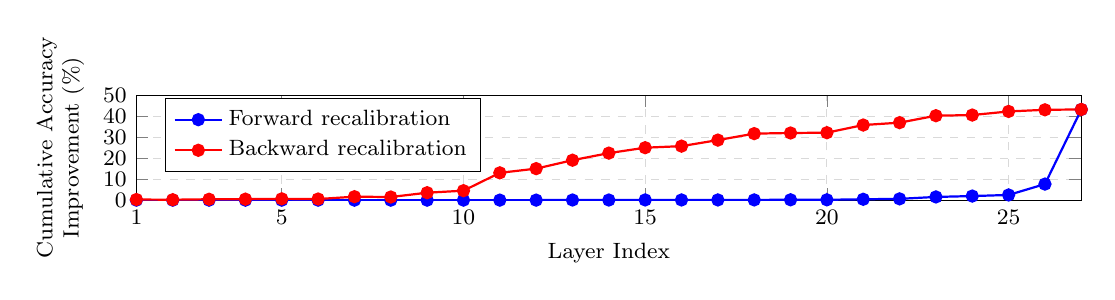
\begin{tikzpicture}
    \begin{axis}[
        width=12cm,
        height=0.11\textwidth,
        scale only axis,
        grid=major,
        grid style={dashed,gray!30},
        tick label style={font=\footnotesize},
        label style={font=\footnotesize},
        legend style={font=\footnotesize},
        cycle list name=color list,
        legend cell align=left,
        xlabel={Layer Index},
        ylabel style={align=center},
        ylabel={Cumulative Accuracy \\Improvement (\%)},
        xmin=1, xmax=27,
        ymin=0, ymax=50,
        xtick={1, 5, 10, 15, 20, 25},
        ytick={0, 10, 20, 30, 40, 50},
        legend pos=north west
    ]

    % Forward recalibration data
    \addplot[color=blue, mark=*, solid, thick] coordinates {
        (1, 0.0)
        (2, -0.0)
        (3, -0.0)
        (4, 0.0)
        (5, 0.0)
        (6, -0.0)
        (7, -0.0)
        (8, -0.0)
        (9, 0.01)
        (10, 0.02)
        (11, 0.02)
        (12, 0.02)
        (13, 0.08)
        (14, 0.07)
        (15, 0.11)
        (16, 0.1)
        (17, 0.11)
        (18, 0.12)
        (19, 0.18)
        (20, 0.17)
        (21, 0.42)
        (22, 0.62)
        (23, 1.54)
        (24, 1.95)
        (25, 2.48)
        (26, 7.65)
        (27, 43.15)
    };

    % Backward recalibration data
    \addplot[color=red, mark=*, solid, thick] coordinates {
        (1, 0.3)
        (2, 0.21)
        (3, 0.43)
        (4, 0.48)
        (5, 0.63)
        (6, 0.54)
        (7, 1.65)
        (8, 1.5)
        (9, 3.55)
        (10, 4.51)
        (11, 13.01)
        (12, 15.01)
        (13, 19.02)
        (14, 22.4)
        (15, 24.98)
        (16, 25.72)
        (17, 28.6)
        (18, 31.68)
        (19, 31.98)
        (20, 32.12)
        (21, 35.77)
        (22, 36.9)
        (23, 40.21)
        (24, 40.52)
        (25, 42.24)
        (26, 43.02)
        (27, 43.19)
    };

    \legend{Forward recalibration, Backward recalibration}
    \end{axis}
\end{tikzpicture}
\caption{Cumulative accuracy improvement (\%) for MobileNet at 80\% sparsity after one-shot magnitude pruning. Forward recalibration progresses from the first BN layer to the last, while backward recalibration starts from the last BN layer. Backward recalibration achieves significant improvements earlier than forward recalibration, reflecting the higher sensitivity of deeper layers to pruning-induced changes.}\label{fig:layerwise_recovery}
\end{figure}






\subsection{Effect of Batch Size on Performance}\label{sec:Ablation_batch}

Here, we investigate the influence of varying batch sizes on the test accuracy of \REFLOW{} for different target sparsity levels (\(\kappa\)) as shown in Figure~\ref{fig:batch_acc}. 


\begin{figure}[t]
\centering
\begin{tikzpicture}
    \begin{groupplot}[
        group style={
            group size=5 by 1,
            vertical sep=35pt,
            horizontal sep=18pt
        },
        width=2.5cm,
        height=0.1\textwidth,
        scale only axis,
        grid=major,
        grid style={dashed,gray!30},
        tick label style={font=\footnotesize},
        label style={font=\footnotesize},
        legend style={font=\footnotesize},
        cycle list name=color list,
        legend cell align=left,
        xmode=log, % Set x-axis to logarithmic
        log basis x={2}, % Use base 2 for logarithmic calculations
        xmin=1, xmax=256,
        ymin=-5, ymax=80,
        xtick={1,2,4,8,16,32,64,128,256},
        xlabel near ticks,
        ylabel near ticks,
    ]
    
    \nextgroupplot[title={$\kappa = 0.4$}, ylabel={Accuracy (\%)}, xlabel={Batch size}, title style={font=\footnotesize}]
    \addplot[color=olive, mark=*] coordinates {
    (1.0, 48.97) (2.0, 63.05) (4.0, 69.38) (8.0, 70.30) (16.0, 71.28) (32.0, 71.29) (64.0, 71.42) (128.0, 71.46) (256.0, 71.48)
    };
    \addplot[color=black, dashed] coordinates {
    (1.0, 69.16) (256.0, 69.16)
    };

    \nextgroupplot[title={$\kappa = 0.5$}, xlabel={Batch size}, title style={font=\footnotesize}]
    \addplot[color=green, mark=*] coordinates {
    (1.0, 49.45) (2.0, 64.52) (4.0, 67.57) (8.0, 69.40) (16.0, 69.97) (32.0, 70.31) (64.0, 70.45) (128.0, 70.53) (256.0, 70.55)
    };
    \addplot[color=black, dashed] coordinates {
    (1.0, 62.61) (256.0, 62.61)
    };

    \nextgroupplot[title={$\kappa = 0.6$}, xlabel={Batch size}, title style={font=\footnotesize}]
    \addplot[color=blue, mark=*] coordinates {
    (1.0, 40.52) (2.0, 58.38) (4.0, 64.25) (8.0, 66.64) (16.0, 67.31) (32.0, 67.54) (64.0, 67.63) (128.0, 67.66) (256.0, 67.66)
    };
    \addplot[color=black, dashed] coordinates {
    (1.0, 41.94) (256.0, 41.94)
    };

    \nextgroupplot[title={$\kappa = 0.7$}, xlabel={Batch size}, title style={font=\footnotesize}]
    \addplot[color=magenta, mark=*] coordinates {
    (1.0, 34.30) (2.0, 50.54) (4.0, 57.34) (8.0, 59.93) (16.0, 60.55) (32.0, 61.14) (64.0, 61.22) (128.0, 61.36) (256.0, 61.43)
    };
    \addplot[color=black, dashed] coordinates {
    (1.0, 6.78) (256.0, 6.78)
    };

    \nextgroupplot[title={$\kappa = 0.8$}, xlabel={Batch size}, title style={font=\footnotesize}]
    \addplot[color=orange, mark=*] coordinates {
    (1.0, 19.80) (2.0, 31.55) (4.0, 38.26) (8.0, 41.28) (16.0, 42.50) (32.0, 42.99) (64.0, 42.95) (128.0, 43.27) (256.0, 43.33)
    };
    \addplot[color=black, dashed] coordinates {
    (1.0, 0.11) (256.0, 0.11)
    };

    \end{groupplot}
\end{tikzpicture}
\caption{Test accuracy of MobileNet at different sparsity levels (\(\kappa\)) and varying batch sizes on ImageNet using \REFLOW{}. Dashed lines represent the baseline accuracy for Magnitude Pruning (MP) without \REFLOW{}.}
\label{fig:batch_acc}
\end{figure}



At lower sparsity levels (\(\kappa = 0.4\) and \(\kappa = 0.5\)), using smaller batch sizes for \REFLOW{} results in a drop in accuracy below the baseline performance of Magnitude Pruning (MP). This indicates that insufficient recalibration data can negatively impact performance in less sparse networks. However, increasing the batch size leads to a noticeable improvement in accuracy, with \REFLOW{} surpassing MP at moderate and large batch sizes. These results demonstrate that networks with lower sparsity still benefit from recalibration when sufficient batch statistics are available.

For intermediate sparsity (\(\kappa = 0.6\)), the impact of batch size is more pronounced. Accuracy improves consistently with larger batch sizes, significantly outperforming MP even at smaller batch sizes. Saturation occurs at moderate batch sizes, highlighting the increased dependency on recalibration as network sparsity increases.

At higher sparsity levels (\(\kappa = 0.7\) and \(\kappa = 0.8\)), larger batch sizes are critical for achieving substantial gains over MP. Accuracy improves steadily with batch size, with saturation occurring at higher batch sizes compared to lower sparsity levels. These results highlight the importance of recalibration in mitigating the performance degradation caused by high sparsity. The dashed lines in Figure~\ref{fig:batch_acc} provide a reference to the baseline MP performance, underscoring the effectiveness of \REFLOW{} in recovering accuracy, particularly for highly sparse networks.




\section{Analyzing Pruning Similarity Using Hamming Distance}\label{appendix:pruning_similarity}
To further understand the limited role of weight selection, we analyze the  \textit{Normalized Hamming Distance} between pruning masks produced by MP, CHITA, and random pruning. CHITA is used as the representative state-of-the-art (SOTA) IP method.

The \textit{Hamming Distance} between two masks \( m^{(A)} \) and \( m^{(B)} \) is defined as:
\[
H(m^{(A)}, m^{(B)}) = \sum_{i=1}^d \mathbb{I}\left(m^{(A)}_i \neq m^{(B)}_i\right),
\]
where \( \mathbb{I}(\cdot) \) is the indicator function, \( d \) is the total number of parameters, and \( m_i = 1 \) indicates that parameter \( i \) is retained. The \textit{Normalized Hamming Distance}, which measures the fraction of differing pruning decisions between two masks, is defined as:  
\[
H_{\text{norm}}(m^{(A)}, m^{(B)}) = \frac{H(m^{(A)}, m^{(B)})}{d}.
\]
where \( H(m^{(A)}, m^{(B)}) \) is the Hamming Distance, and \( d \) is the total number of parameters.


Figure~\ref{fig:normalized_hamming} shows that the Normalized Hamming Distance between MP and CHITA is negligible, indicating close similarity in their pruning decisions compared to the significant variation with random pruning. For ResNet-20 on CIFAR-10, it is \(0.0018\%\). For MobileNet on ImageNet, it is \(0.0095\%\). These results show that magnitude-based and IP-selection methods make nearly identical pruning decisions, supporting the conclusion that the choice of weight selection (MP or IP-selection) has minimal influence on pruning performance.

\begin{figure}[h]
\centering
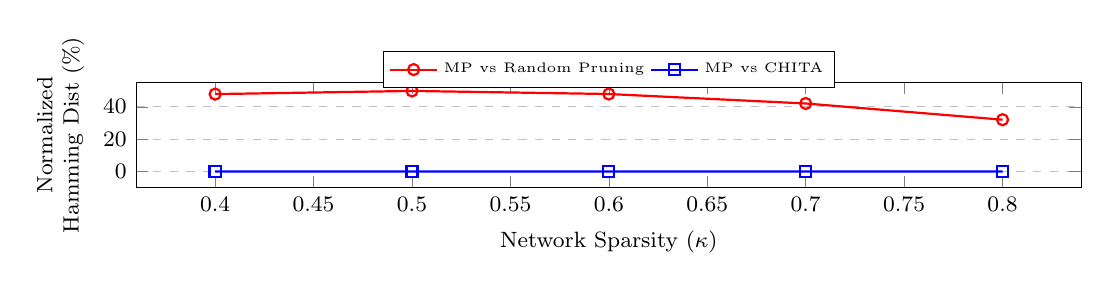
\begin{tikzpicture}
\begin{axis}[
    width=12cm,
    height=0.11\textwidth,
    scale only axis,
    xlabel={Network Sparsity (\(\kappa\))},
    ylabel={Normalized \\ Hamming Dist (\%)},
    ylabel style={align=center},
    ymin=-10, ymax=55,
    ymajorgrids=true,
    grid style=dashed,
    legend pos=south east,
    legend style={
        at={(0.5,+1.3)},
        anchor=north,
        font=\tiny,
        cells={anchor=west},
        inner sep=2pt,
        legend columns=4,
    },
    ymajorgrids=true,
    grid style=dashed,
    tick label style={font=\footnotesize},
    label style={font=\footnotesize},
    legend cell align=left,
    mark options={scale=1},
    cycle list name=color list
]

% Normalized Hamming Distance MP vs Random Pruning
\addplot[color=red, mark=o, solid, thick] coordinates {
    (0.4, 47.8897)
    (0.5, 49.8520)
    (0.6, 47.9436)
    (0.7, 42.0788)
    (0.8, 32.0510)
};
\addlegendentry{MP vs Random Pruning}

% Normalized Hamming Distance MP vs CHITA
\addplot[color=blue, mark=square, solid, thick] coordinates {
    (0.4, 0.0018)
    (0.5, 0.0018)
    (0.6, 0.0022)
    (0.7, 0.0030)
    (0.8, 0.0030)
};
\addlegendentry{MP vs CHITA}

\end{axis}
\end{tikzpicture}
\caption{Normalized Hamming Distance (\%) between pruning masks for Magnitude Pruning (MP) vs Random pruning and MP vs CHITA across sparsity levels. MP and CHITA have negligible variation, while MP and Random pruning show significant differences.}
\label{fig:normalized_hamming}
\end{figure}